%\title{LaTeX Portrait Poster Template}
%%%%%%%%%%%%%%%%%%%%%%%%%%%%%%%%%%%%%%%%%
% a0poster Portrait Poster
% LaTeX Template
% Version 1.0 (22/06/13)
%
% The a0poster class was created by:
% Gerlinde Kettl and Matthias Weiser (tex@kettl.de)
% 
% This template has been downloaded from:
% http://www.LaTeXTemplates.com
%
% License:
% CC BY-NC-SA 3.0 (http://creativecommons.org/licenses/by-nc-sa/3.0/)
%
%%%%%%%%%%%%%%%%%%%%%%%%%%%%%%%%%%%%%%%%%

%----------------------------------------------------------------------------------------
%	PACKAGES AND OTHER DOCUMENT CONFIGURATIONS
%----------------------------------------------------------------------------------------

\documentclass[a0,portrait]{a0poster}

\usepackage{multicol} % This is so we can have multiple columns of text side-by-side
\columnsep=100pt % This is the amount of white space between the columns in the poster
\columnseprule=3pt % This is the thickness of the black line between the columns in the poster

\usepackage[svgnames]{xcolor} % Specify colors by their 'svgnames', for a full list of all colors available see here: http://www.latextemplates.com/svgnames-colors

\usepackage{times} % Use the times font
%\usepackage{palatino} % Uncomment to use the Palatino font

\usepackage{graphicx} % Required for including images
\graphicspath{{figures/}} % Location of the graphics files
\usepackage{booktabs} % Top and bottom rules for table
\usepackage[font=small,labelfont=bf]{caption} % Required for specifying captions to tables and figures
\usepackage{amsfonts, amsmath, amsthm, amssymb} % For math fonts, symbols and environments
\usepackage{wrapfig} % Allows wrapping text around tables and figures
\usepackage[brazilian]{babel}
\usepackage[utf8]{inputenc}
\usepackage[T1]{fontenc}
\usepackage{float}
\usepackage[most]{tcolorbox}

\definecolor{DeepOrange}{HTML}{ff690a}

\begin{document}

%----------------------------------------------------------------------------------------
%	POSTER HEADER 
%----------------------------------------------------------------------------------------

% The header is divided into two boxes:
% The first is 75% wide and houses the title, subtitle, names, university/organization and contact information
% The second is 25% wide and houses a logo for your university/organization or a photo of you
% The widths of these boxes can be easily edited to accommodate your content as you see fit

\begin{minipage}[b]{0.75\linewidth}
\veryHuge \color{DeepOrange} \textbf{USPCodeLab} \color{Black}\\ [1cm]% Title
\Huge Atividade Curricular em Cultura e Extensão\\[2cm] % Subtitle
\huge \textbf{Leonardo Lana Violin Oliveira}\\[0.5cm] % Author(s)
\textbf{Orientador: Renato Cordeiro}\\[0.5cm] % Author(s)
\huge Universidade de São Paulo\\[0.4cm] % University/organization
\Large \texttt{leolanavo@gmail.com} \\
\end{minipage}
%
\begin{minipage}[b]{0.25\linewidth}
\includegraphics[width=20cm]{UCL-Logo-660px.png}\\
\end{minipage}

\vspace{1cm} % A bit of extra whitespace between the header and poster content

%----------------------------------------------------------------------------------------

\begin{multicols}{2} % This is how many columns your poster will be broken into, a portrait poster is generally split into 2 columns

\begin{tcolorbox}[ breakable,
                   coltext=white,
                   colback=DeepOrange,
                   colframe=DeepOrange,
                   width=36cm,
                   top=0.3cm,
                   enlarge left by=-6mm]
    \section*{Introdução}
\end{tcolorbox}

Durante este semestre desenvolvi 100 horas de atividades no grupo USPCodeLab,
estas 100 horas foram dividadas entre: a organização do HackathonUSP 2018.1, incluindo
realização da licitação para o fornecimento da alimentação do evento, arrumação do local do evento, 
negociação com patrocinadores, e permanência durante o evento; a apresentação e organização do
\textsc{dev.learn()}, incluindo reformulando o material, apresentando as palestras de HTML, CSS e JS; treinamento dos novos membros da 
organização do USPCodeLab, incluindo criar o manual para novos membros da organização, montar as 
equipes para cuidar  das múltiplas tarefas do grupo. \\[0.5cm]

%----------------------------------------------------------------------------------------
%	OBJECTIVES
%----------------------------------------------------------------------------------------


\begin{tcolorbox}[ breakable,
                   coltext=white,
                   colback=DeepOrange,
                   colframe=DeepOrange,
                   width=36cm,
                   top=0.3cm,
                   enlarge left by=-6mm]
\section*{Principais Objetivos}
\end{tcolorbox}

\subsection*{HackathonUSP 2018.1}
\begin{enumerate}
    \item Realizar um evento que seja ao mesmo tempo acessível a iniciantes, porém que somente estudantes
    experientes sejam premiados
    
    \item Aproveitar a empolgação para o evento para realizar um curso preparatório para
    capacitação dos participantes e captar membros para os grupos de estudos do USPCodeLab
    
    \item Agrupar os projetos mais interessantes e apresentá-los para a Pró-Reitoria de Pesquisa
    para que, caso haja interesse dos alunos e da Pró-Reitoria de Pesquisa, estes projetos sejam
    implementados
\end{enumerate}

\subsection*{dev.learn()}
\begin{enumerate}
    \item Ensinar aos alunos do curso o básico de programação web, ou seja, HTML, CSS e JS
    puros.
   
    \item Mostrar aos alunos a importância da escolha de ferramentas no início do desenvolvimento
    de um projeto em grupo e de longa duração
    
    \item Apresentar aos alunos técnicas de desenvolvimento ágil
    
    \item Validar o nosso material sobre web básico em um ambiente adverso e utilizarmos o feedback
    para melhorar o material ainda mais
\end{enumerate}

\subsection*{Treinamento de novos membros da organização}
\begin{enumerate}
    \item Treinar novos membros para que mesmo após os membros fundadores saírem do grupo
    o grupo continue com suas atividades
    
    \item Os novos membros formaram times para que o grupo expanda suas atividades nas mídias
    sociais, de desenvolvimento de projetos, organização de eventos e realização dos cursos\\[0.5cm]
\end{enumerate} 

%----------------------------------------------------------------------------------------
%	HACKATHONUSP 2018.1
%----------------------------------------------------------------------------------------

\begin{tcolorbox}[ breakable,
                   coltext=white,
                   colback=DeepOrange,
                   colframe=DeepOrange,
                   width=36cm,
                   top=0.3cm,
                   bottom=0.4cm,
                   enlarge left by=-6mm]
    \section*{Resumo das atividades}
\end{tcolorbox}

\subsection*{HackathonUSP 2018.1}

\subsubsection*{Arrumação para o local do evento}
Para a arrumação do local o time do USPCodeLab moveu 27 mesas, 300 cadeiras foram movidas 
entre os blocos e salas do IME.

\subsubsection*{Negociação com patrocinadores}
Para a realização do evento foi necessário além do patrocínio da PRP (Pró-Reitoria da Pesquisa),
o patrocínio de empresas privadas, para este primeiro evento só contatei a VTEX. Para o firmamento
da parceira foi necessário a elaboração de um contrato.

\subsubsection*{Permanência durante o evento}
Durante o evento, fiquei responsável pela liderança do time de 10 pessoas do USPCodeLab, 
dividi a equipe em pequenos times para cuidar de cada tarefa: finalizar a instalação
elétrica, limpar as salas, montar o ambiente do evento, preparar a sala
para a empresa que forneceu a comida.

\subsection*{dev.learn()}
\subsubsection*{Apresentação das palestras}
No início de \textsc{dev.learn()} há o oferecimento do \textsc{dev.start()}, que é o ciclo
de palestras de web básico, apresentando temas como HTML, CSS e JS, com o objetivo de 
capacitar os alunos a entender as documentações disponibilizadas online.

\subsubsection*{Reformulação do material}
Reformulamos o material de web básico, atualizando o material para as novas especificações
lançadas pós 2015. Incluímos tags semânticas e outras novidades do HTML5, ferramentas
para definição de layout em CSS, incluímos \textit{arrow functions} e \textit{querySelector}
e retiramos \textit{JQuerry} em JS.

\subsection*{Treinamento de novos membros da organização}
\subsubsection*{Criação do manual}
Para orientação dos novos membros foi criado para um manual explicando quais as funções de
cada time, como o nosso canal de comunicação funciona e como a organização em geral trabalha.

\subsubsection*{Criação das equipes}
No final do ano passado, ingressaram 10 novos membros então pude dividir a organização em
4 times, cada um cuidando de uma parte do grupo, os time são: relações públicas, eventos,
\textsc{dev.journey()} e projetos.\\[0.5cm]

%----------------------------------------------------------------------------------------
%	RESULTS 
%----------------------------------------------------------------------------------------

\begin{tcolorbox}[ breakable,
                   coltext=white,
                   colback=DeepOrange,
                   colframe=DeepOrange,
                   width=36cm,
                   top=0.3cm,
                   bottom=0.4cm,
                   enlarge left by=-6mm]
\section*{Resultados}
\end{tcolorbox}

\subsection*{HackathonUSP 2018.1}
Com o HackathonUSP 2018.1 alcançamos 365 inscritos, com a participação de 81 alunos da USP de
8 institutos diferentes da USP.

Tivemos nosso evento divulgado por entidades USPianas, como o JornalUSP e o Jornal do IME. Além
disso, tivemos reportagens na mídia externa à USP, o evento foi exibido em uma matéria durante
o Bom Dia São Paulo.

\begin{figure}[H]
    \centering
    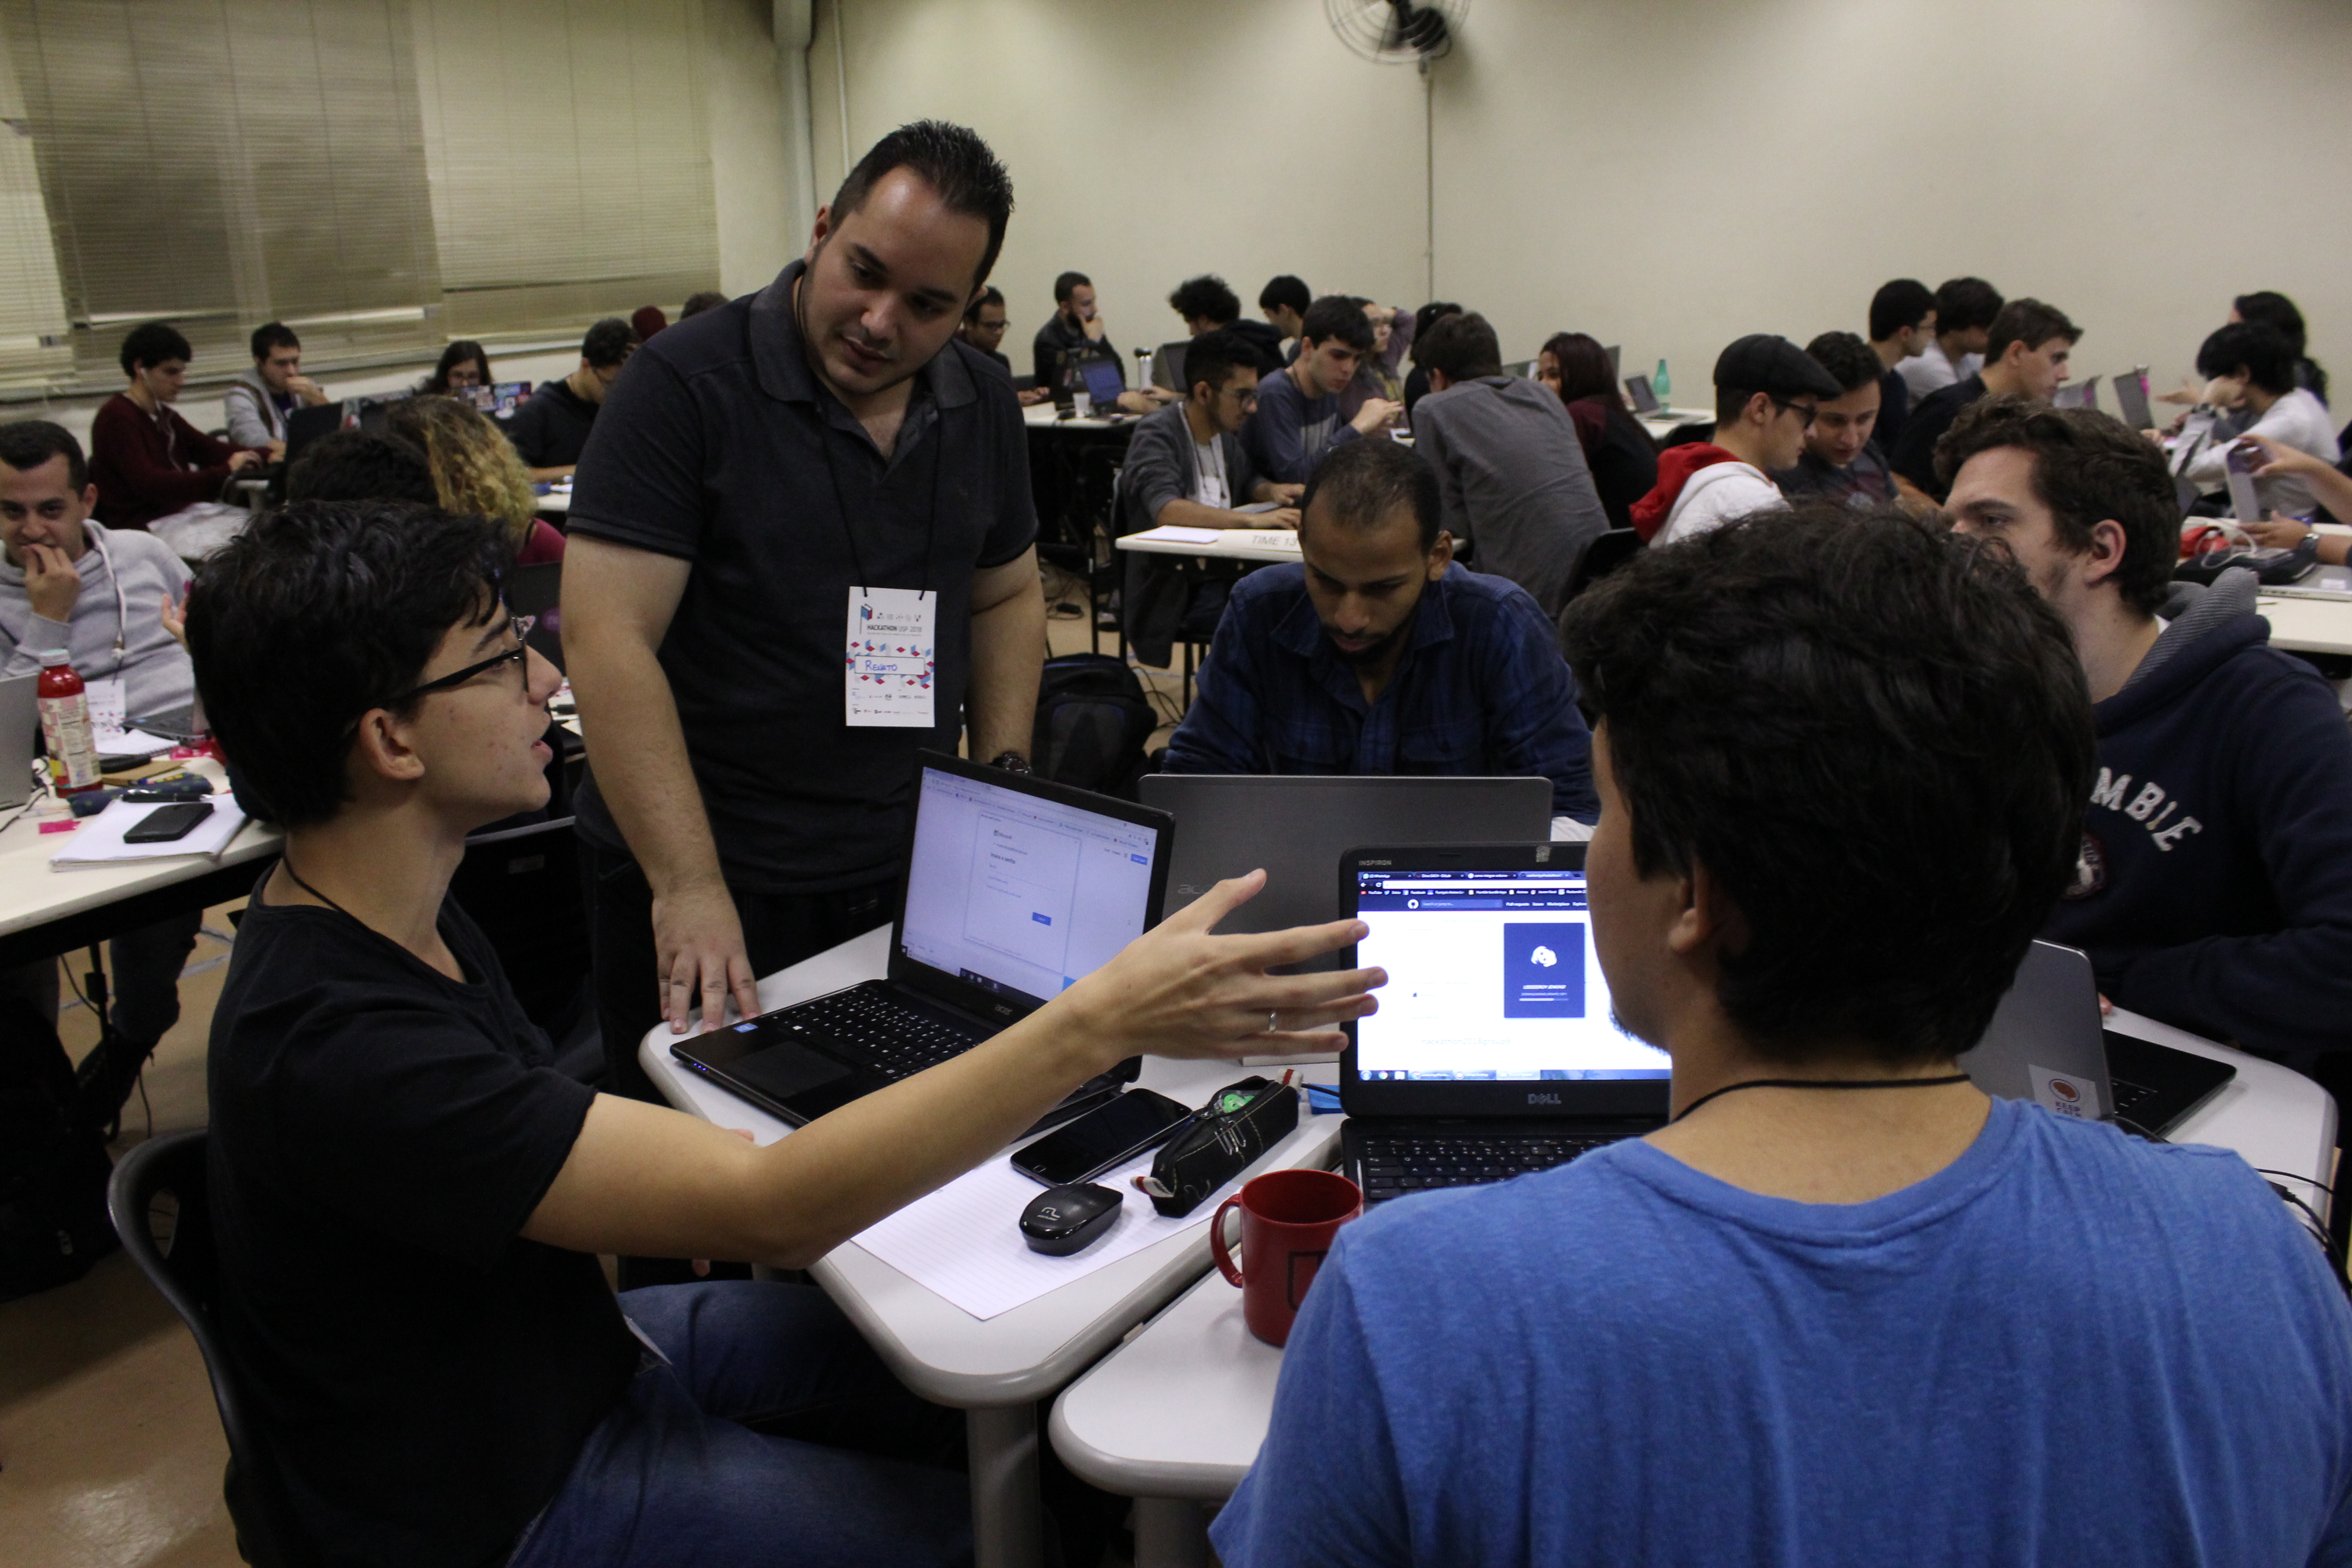
\includegraphics[width=500px]{IMG_7796.JPG}
    \caption{HackathonUSP 2018.1}
\end{figure}

\subsection*{dev.learn()}
Tivemos uma turma de 14 alunos que aprenderam o básico de HTML, CSS e JS, e hoje em dia estão
desenvolvendo uma aplicação web que cataloga os heróis da Marvel usando requesições HTTP para a
API da emrpesa.

\begin{figure}[H]
    \centering
    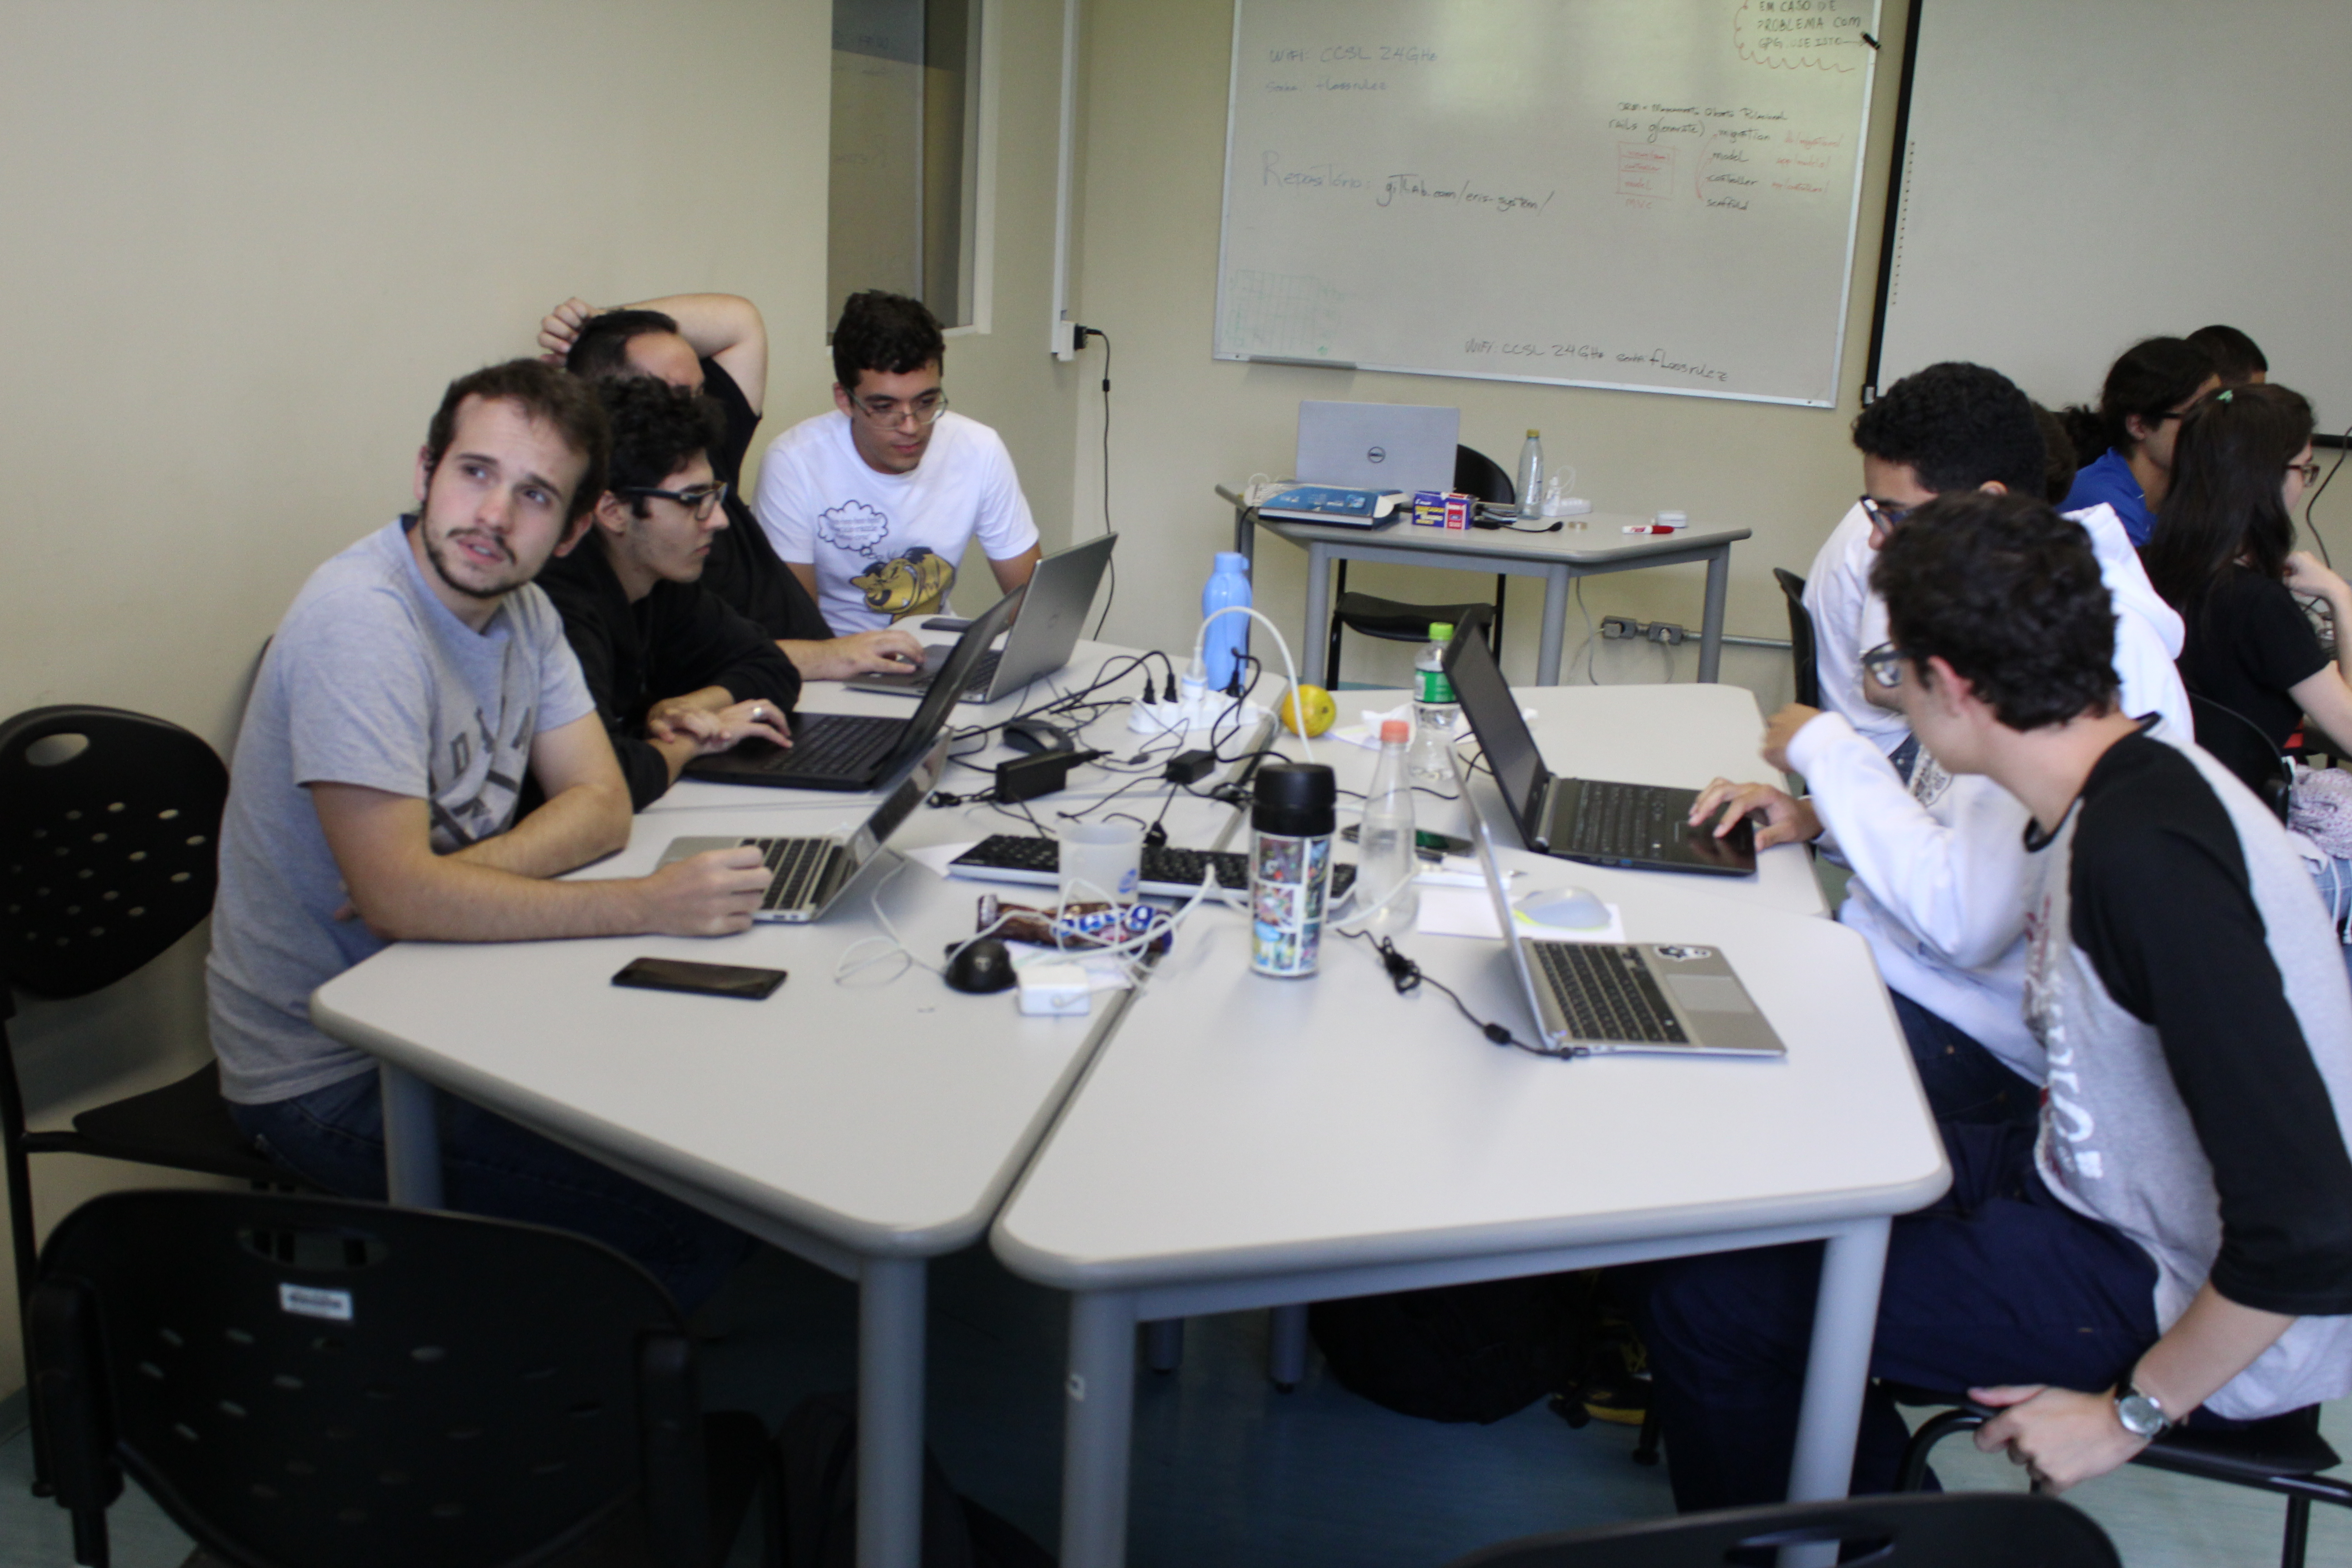
\includegraphics[width=500px]{IMG_7164.JPG}
    \caption{dev.learn()}
\end{figure}

\subsection*{Treinamento de novos membros da organização}
Foi gerado o manual de novos membros da organização, diminuindo o atrito da inserção de um novo 
membro em nosso time significativamente.
Durante este semestre passamos de 2 pessoas no time para 13 pessoas no time divididas entre
4 times.

\begin{figure}[H]
    \centering
    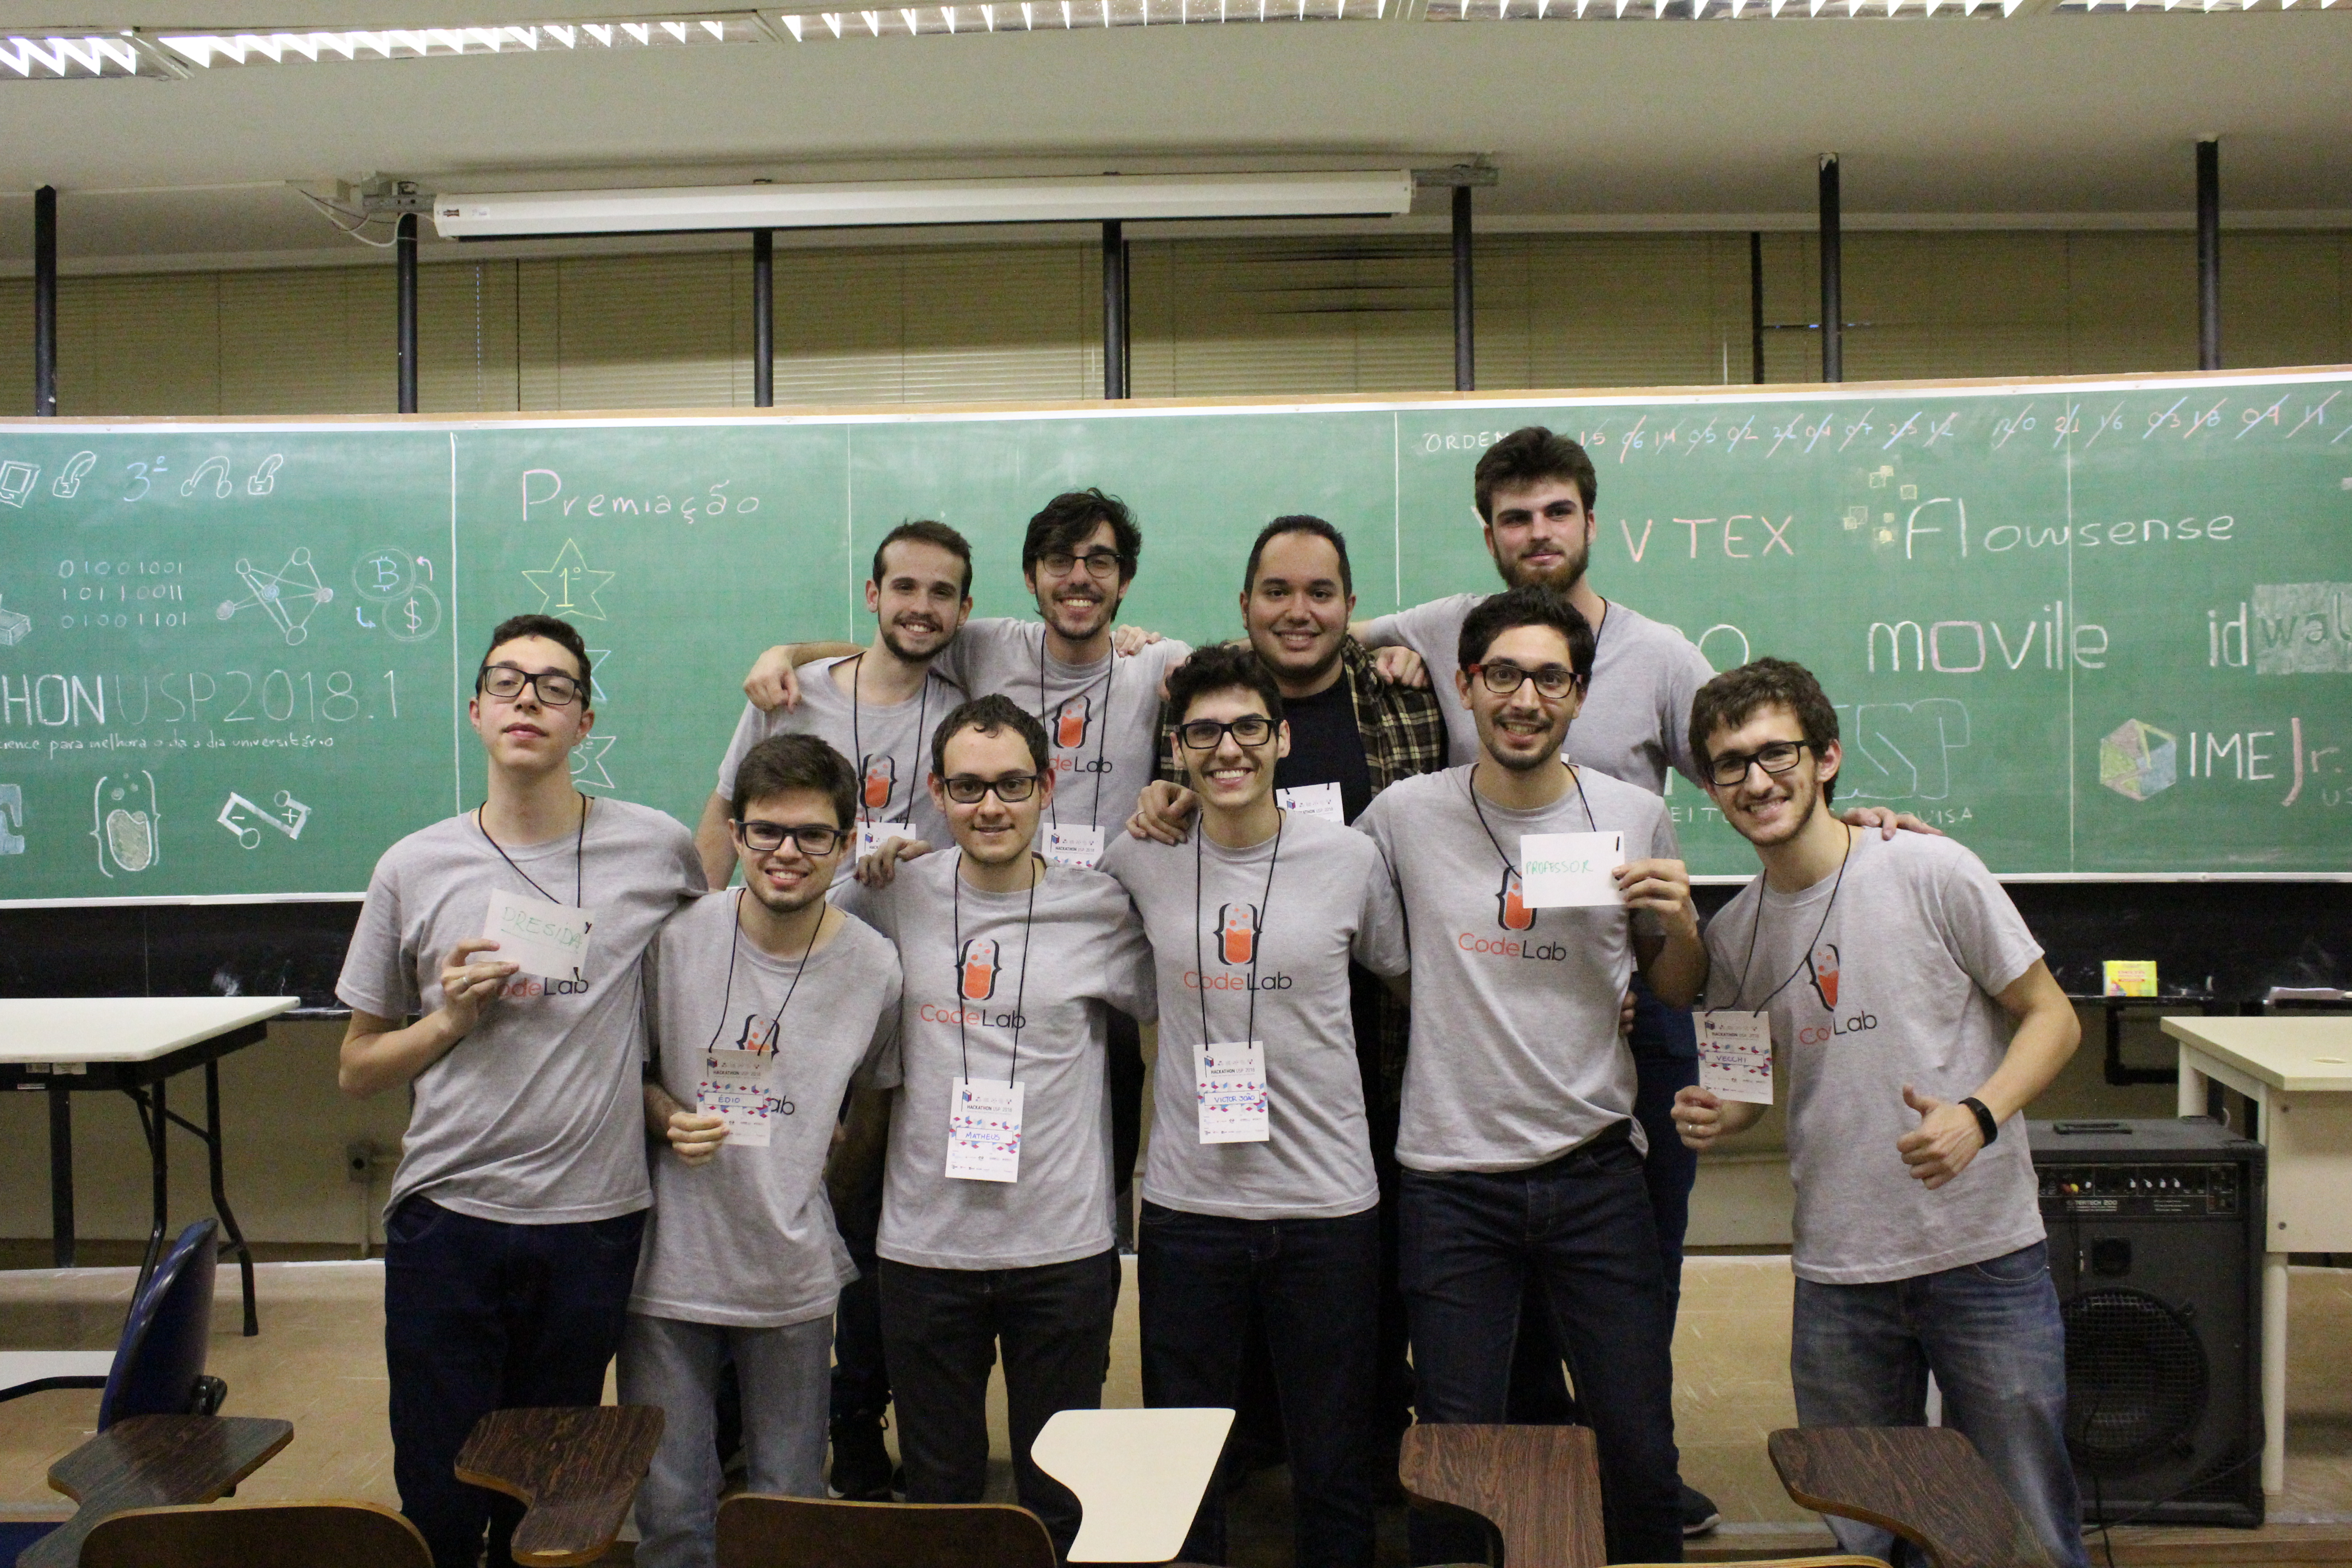
\includegraphics[width=500px]{IMG_8020.JPG}
    \caption{Organização com os novos membros}
\end{figure}

\begin{tcolorbox}[ breakable,
                   coltext=white,
                   colback=DeepOrange,
                   colframe=DeepOrange,
                   width=36cm,
                   top=0.3cm,
                   bottom=0.4cm,
                   enlarge left by=-6mm]
    \section*{Horas gastas}
\end{tcolorbox}

\begin{table}[H]
\centering
\label{my-label}
\begin{tabular}{|l|r|}
\hline
\textbf{Atividade}               & \multicolumn{1}{l|}{\textbf{Horas gastas}} \\ \hline
Arrumação do local do evento     & 10                                         \\ \hline
Negociação com os patrocinadores & 16                                         \\ \hline
Permanência durante o evento     & 24                                         \\ \hline
Apresentação das palestras       & 12                                         \\ \hline
Reformulação do material         & 12                                         \\ \hline
Criação do manual                & 10                                         \\ \hline
Criação das equipes              & 16                                         \\ \hline
\end{tabular}
\end{table}

\end{multicols}
\end{document}